%\newcommand{\nm}[1] {\hline\multicolumn{1}{c}{\cellcolor{black} { {\bf \textcolor{white}{#1}}}}}
\pdfoutput=1
\newcommand{\nm}[1] { \hline &\multicolumn{1}{l}{  {\bf #1 }}}


\newcommand{\ofr} {
{\textit{out-of-range}}
}
\newcommand{\quart}[4]{\begin{picture}(100,3)%1
{\color{black}\put(#3,3){\circle*{4}}\put(#1,3){\line(1,0){#2}}}\end{picture}}

\begin{figure*}[!thbp]
 \setlength{\belowcaptionskip}{-16pt}
 
\begin{center}
\renewcommand{\baselinestretch}{0.65} 
\begin{minipage}{0.45\linewidth}
% \resizebox{\linewidth}{!}{
% %\begin{tabular}{l@{~~~~}l@{~~~~}r@{~~~~}r@{~~}c@{}}
% \begin{tabular}{llrrc}
%   {\textbf{Rank}}& \textbf{Using} & \textbf{Med.} & \textbf{IQR} & \\ 
  
  
%   %%% generating from latex_plotting.py::plot_mre_for_all
% \nm{kemerer}\\
%     1 &      DE8 &    21 &  32 & \quart{15}{32}{21}{100} \\
%   \rowcolor{black!10}   1* &      DE2 &    22 &  27 & \quart{16}{27}{22}{100} \\
%     1 &      RANDOM160 &    24 &  17 & \quart{19}{17}{24}{100} \\
%   \rowcolor{black!10}   1* &      RANDOM40 &    26 &  27 & \quart{17}{27}{26}{100} \\
%     2 &      ABE0 &    60 &  53 & \quart{17}{53}{60}{100} \\
%     3 &      ATLM &    154 &  341 & \ofr \\ %\quart{96}{341}{154}{100} \\
% \nm{albrecht}\\
%     1 &      DE8 &    19 &  6 & \quart{15}{6}{19}{100} \\
%  \rowcolor{black!10}   1* &      DE2 &    21 &  6 & \quart{18}{6}{21}{100} \\
%     1 &      RANDOM160 &    24 &  12 & \quart{19}{12}{24}{100} \\
%     2 &      RANDOM40 &    28 &  16 & \quart{26}{16}{28}{100} \\
%     3 &      ABE0 &    48 &  34 & \quart{30}{34}{48}{100} \\
%     4 &      ATLM &    97 &  76 & \ofr \\%\\\quart{59}{76}{97}{100} \\
% \nm{isbsg10}\\
%     1 &      DE8 &    37 &  43 & \quart{30}{43}{37}{100} \\
%   \rowcolor{black!10}    1* &      DE2 &    43 &  22 & \quart{38}{22}{43}{100} \\
%     2 &      RANDOM160 &    48 &  21 & \quart{41}{21}{48}{100} \\
%     2 &      RANDOM40 &    56 &  24 & \quart{47}{24}{56}{100} \\
%     2 &      ABE0 &    72 &  22 & \quart{53}{22}{72}{100} \\
%     3 &      ATLM &    138 &  120 &  \ofr %\quart{94}{120}{138}{100}
%     \\
% \nm{finnish}\\
%     1 &      DE2 &    15 &  18 & \quart{9}{18}{15}{100} \\
%   \rowcolor{black!10}   1* &      ATLM &    18 &  9 & \quart{14}{9}{18}{100} \\
%     1 &      RANDOM160 &    21 &  18 & \quart{13}{18}{21}{100} \\
%     2 &      DE8 &    22 &  30 & \quart{10}{30}{22}{100} \\
%     2 &      RANDOM40 &    24 &  18 & \quart{16}{18}{24}{100} \\
%     3 &      ABE0 &    37 &  19 & \quart{33}{19}{37}{100} \\
% \nm{miyazaki}\\
%     1 &      DE8 &    21 &  33 & \quart{10}{33}{21}{100} \\
%   \rowcolor{black!10}   1* &      DE2 &    21 &  31 & \quart{13}{31}{21}{100} \\
%     1 &      RANDOM160 &    23 &  25 & \quart{16}{25}{23}{100} \\
%   \rowcolor{black!10}   1* &      RANDOM40 &    31 &  22 & \quart{19}{22}{31}{100} \\
%     2 &      ABE0 &    56 &  16 & \quart{46}{16}{56}{100} \\
%     3 &      ATLM &    147 &  98 & \ofr %
%     \\%\quart{91}{98}{147}{100} \\
% \nm{maxwell}\\
%     1 &      DE8 &    28 &  32 & \quart{18}{32}{28}{100} \\
%   \rowcolor{black!10}   1* &      DE2 &    28 &  20 & \quart{19}{20}{28}{100} \\
%     2 &      RANDOM160 &    34 &  26 & \quart{26}{26}{34}{100} \\
%     3 &      RANDOM40 &    40 &  19 & \quart{31}{19}{40}{100} \\
%     3 &      ABE0 &    55 &  26 & \quart{39}{26}{55}{100} \\
%     4 &      ATLM &    357 &  322 & \ofr \\ %\quart{204}{322}{357}{100} \\
% \nm{desharnais}\\
%     1 &      DE8 &    24 &  28 & \quart{14}{28}{24}{100} \\
%   \rowcolor{black!10}  1* &      DE2 &    24 &  20 & \quart{18}{20}{24}{100} \\
%     1 &      RANDOM160 &    28 &  15 & \quart{21}{15}{28}{100} \\
%     2 &      RANDOM40 &    32 &  19 & \quart{24}{19}{32}{100} \\
%     3 &      ATLM &    47 &  23 & \quart{36}{23}{47}{100} \\
%     3 &      ABE0 &    52 &  27 & \quart{40}{27}{52}{100} \\
% \nm{kitchenham}\\
%     1 &      DE8 &    18 &  19 & \quart{14}{19}{18}{100} \\
%   \rowcolor{black!10}  1* &      DE2 &    18 &  12 & \quart{15}{12}{18}{100} \\
%     1 &      RANDOM160 &    22 &  11 & \quart{17}{11}{22}{100} \\
%   \rowcolor{black!10}   1* &      RANDOM40 &    24 &  12 & \quart{19}{12}{24}{100} \\
%     2 &      ABE0 &    43 &  16 & \quart{38}{16}{43}{100} \\
%     3 &      ATLM &    133 &  59 & \ofr \\%\quart{111}{59}{133}{100} \\
% \nm{china}\\
%     1 &      DE8 &    16 &  11 & \quart{13}{11}{16}{100} \\
%   \rowcolor{black!10}   1* &      DE2 &    16 &  6 & \quart{12}{6}{16}{100} \\
%     2 &      RANDOM160 &    24 &  14 & \quart{18}{14}{24}{100} \\
%     2 &      RANDOM40 &    27 &  17 & \quart{18}{17}{27}{100} \\
%     3 &      ABE0 &    44 &  6 & \quart{40}{6}{44}{100} \\
%     4 &      ATLM &    57 &  14 & \quart{51}{14}{57}{100} \\
% \end{tabular}}
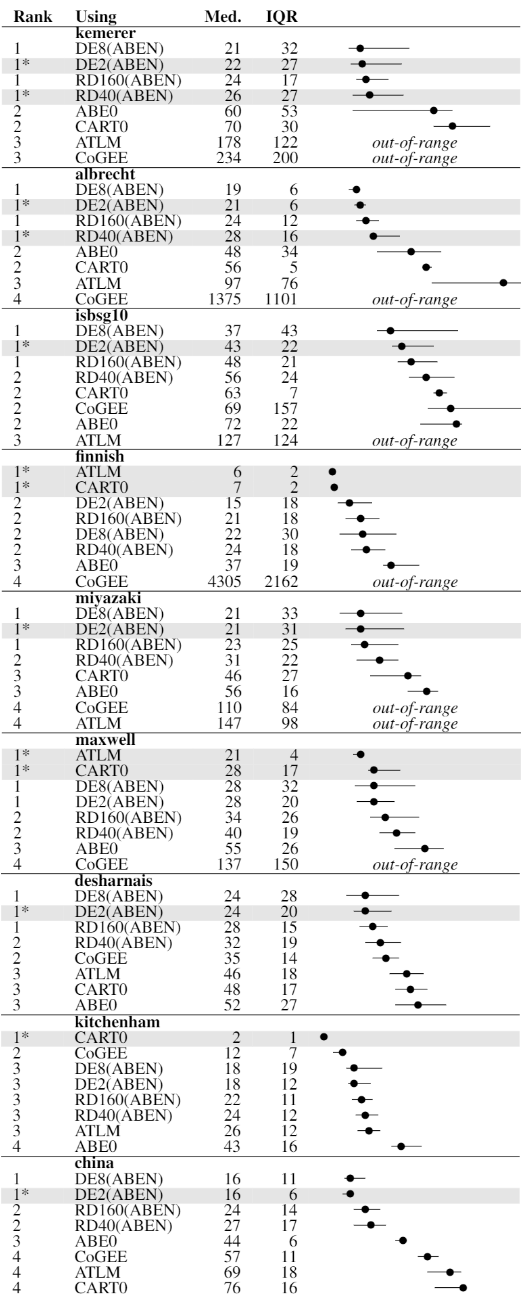
\includegraphics[width=3.3in]{mre.png}
\end{minipage}%
~~%
\begin{minipage}{0.45\linewidth}
\resizebox{\linewidth}{!}{
\begin{tabular}{llrrc}
  {\textbf{Rank}}& \textbf{Using} & \textbf{Med.} & \textbf{IQR} & \\ 
   
    %%% generating from latex_plotting.py::plot_sa_for_all
\nm{kemerer}\\
    1 &      RANDOM160 &    61 &  33 & \quart{38}{33}{61}{100} \\
   \rowcolor{black!10}    1* &      DE2 &    54 &  24 & \quart{43}{24}{54}{100} \\
   \rowcolor{black!10}    1* &      RANDOM40 &    53 &  36 & \quart{33}{36}{53}{100} \\
    1 &      DE8 &    49 &  28 & \quart{41}{28}{49}{100} \\
    2 &      ABE0 &    37 &  51 & \quart{3}{51}{37}{100} \\
    3 &      ATLM &    -46 &  217 & \ofr %\quart{-231}{217}{-46}{100} 
   \\
\nm{albrecht}\\
  \rowcolor{black!10}   1* &      DE8 &    77 &  20 & \quart{64}{20}{77}{100} \\
    2 &      DE2 &    69 &  19 & \quart{61}{19}{69}{100} \\
    2 &      RANDOM160 &    68 &  20 & \quart{56}{20}{68}{100} \\
    3 &      RANDOM40 &    55 &  21 & \quart{44}{21}{55}{100} \\
    3 &      ABE0 &    54 &  38 & \quart{43}{38}{54}{100} \\
    4 &      ATLM &    30 &  50 & \quart{5}{50}{30}{100} \\
\nm{isbsg10}\\
    1 &      RANDOM160 &    40 &  30 & \quart{22}{30}{40}{100} \\
    \rowcolor{black!10}  1* &      ABE0 &    33 &  25 & \quart{23}{25}{33}{100} \\
    1 &      RANDOM40 &    31 &  18 & \quart{22}{18}{31}{100} \\
    1 &      DE8 &    28 &  24 & \quart{22}{24}{28}{100} \\
    1 &      DE2 &    26 &  20 & \quart{22}{20}{26}{100} \\
    2&      ATLM &    10 &  126 & \ofr %\quart{-104}{126}{10}{100}
  \\
\nm{finnish}\\
  \rowcolor{black!10}   1* &      ATLM &    81 &  6 & \quart{77}{6}{81}{100} \\
    1 &      DE2 &    81 &  13 & \quart{74}{13}{81}{100} \\
    1 &      RANDOM160 &    77 &  14 & \quart{70}{14}{77}{100} \\
    2 &      DE8 &    74 &  43 & \quart{44}{43}{74}{100} \\
    2 &      RANDOM40 &    73 &  14 & \quart{65}{14}{73}{100} \\
    3 &      ABE0 &    54 &  25 & \quart{42}{25}{54}{100} \\
\nm{miyazaki}\\
    1 &      RANDOM160 &    60 &  33 & \quart{40}{33}{60}{100} \\
    1 &      DE8 &    57 &  32 & \quart{41}{32}{57}{100} \\
  \rowcolor{black!10}   1* &      DE2 &    57 &  29 & \quart{42}{29}{57}{100} \\
  \rowcolor{black!10}   1* &      RANDOM40 &    55 &  32 & \quart{38}{32}{55}{100} \\
    2 &      ABE0 &    36 &  24 & \quart{25}{24}{36}{100} \\
    3 &      ATLM &    -41 &  85 & \ofr %quart{-87}{85}{-41}{100} 
    \\
\nm{maxwell}\\
    1 &      DE8 &    60 &  26 & \quart{45}{26}{60}{100} \\
    \rowcolor{black!10}   1* &      DE2 &    55 &  34 & \quart{38}{34}{55}{100} \\
    1 &      RANDOM160 &    52 &  26 & \quart{40}{26}{52}{100} \\
  \rowcolor{black!10}   1* &      RANDOM40 &    50 &  26 & \quart{36}{26}{50}{100} \\
    2 &      ABE0 &    41 &  28 & \quart{23}{28}{41}{100} \\
    3 &      ATLM &    -204 &  247 & \ofr\\%\quart{-331}{247}{-204}{100} \\
\nm{desharnais}\\
  \rowcolor{black!10}   1* &      DE2 &    57 &  24 & \quart{44}{24}{57}{100} \\
    1 &      DE8 &    57 &  21 & \quart{47}{21}{57}{100} \\
    2 &      RANDOM160 &    54 &  20 & \quart{41}{20}{54}{100} \\
    2 &      RANDOM40 &    52 &  26 & \quart{37}{26}{52}{100} \\
    2 &      ATLM &    52 &  16 & \quart{41}{16}{52}{100} \\
    3 &      ABE0 &    36 &  17 & \quart{24}{17}{36}{100} \\
\nm{kitchenham}\\
   \rowcolor{black!10}    1* &      RANDOM40 &    67 &  20 & \quart{54}{20}{67}{100} \\
   \rowcolor{black!10}    1* &      DE2 &    66 &  17 & \quart{56}{17}{66}{100} \\
    1 &      RANDOM160 &    66 &  21 & \quart{53}{21}{66}{100} \\
    1 &      DE8 &    65 &  21 & \quart{54}{21}{65}{100} \\
    2 &      ABE0 &    45 &  18 & \quart{35}{18}{45}{100} \\
    3 &      ATLM &    -39 &  72 & \ofr %\quart{-81}{72}{-39}{100}
  \\
\nm{china}\\
    1 &      DE8 &    82 &  11 & \quart{75}{11}{82}{100} \\
    \rowcolor{black!10}   1* &      DE2 &    78 &  12 & \quart{71}{12}{78}{100} \\
    2 &      RANDOM160 &    69 &  19 & \quart{59}{19}{69}{100} \\
    2 &      RANDOM40 &    67 &  27 & \quart{51}{27}{67}{100} \\
    3 &      ABE0 &    60 &  4 & \quart{56}{4}{60}{100} \\
    4 &      ATLM &    41 &  12 & \quart{35}{12}{41}{100} \\
\end{tabular}}

\end{minipage}
\end{center}
 \caption{
\%  {\bf MRE} and \% {\bf SA} seen in 20 repeats.
 {\bf Med} is the 50th percentile and {\bf IQR} is the {\em inter-quartile range}; i.e., 75th-25th percentile. 
    Lines with a dot in the middle (e.g.,\protect\quartex{3}{13}{13}{0})
   show   median values with the IQR.   
   MRE and SA results are sorted in different directions since better MRE and SA values are smaller and larger (respectively).
   The left-hand side columns {\bf Rank} results (and the {\em smaller}, the {\em better}).
    Ranks separate statistically different results, as computed by a bootstrap test (95\% confidence)
   and the A12 test~\cite{Whigham:2015:BMS:2776776.2738037}). \ofr denote
   results that are so bad, that they  fall outside of this figure
   s range of [0,100] \%. 
   \colorbox{black!10}{1*} denotes rows of faster best-ranked methods.}
 \label{fig:jur}
\end{figure*}


